\documentclass[12pt]{scrreprt}

\usepackage[utf8]{inputenc}		% Ermögicht es umlaute direkt zu schreiben
\usepackage{amsmath,amssymb} 	% Mathe symbole und funktionen
\usepackage{graphicx}			% Bilder einbinden
\usepackage[ngerman]{babel} 	% Deutscht alles ein
\usepackage{pdflscape}			% Querformat

\parindent 0px					% Einrückung von absätzen auf 0

\subject{Teilentwurf}
\title{LISE E-Learning System}
\author{Matthias Englert, Fabian Schilha, Andreas Rottach}
\date{Wintersemester 2014/2015}

\begin{document}
\maketitle

\tableofcontents


\chapter{Datenbankentwurf}

\section{Datebankdiagramm}
\begin{figure}[H]
	\centering
	\paragraph{Aufbau der Relationalen Datenbank}	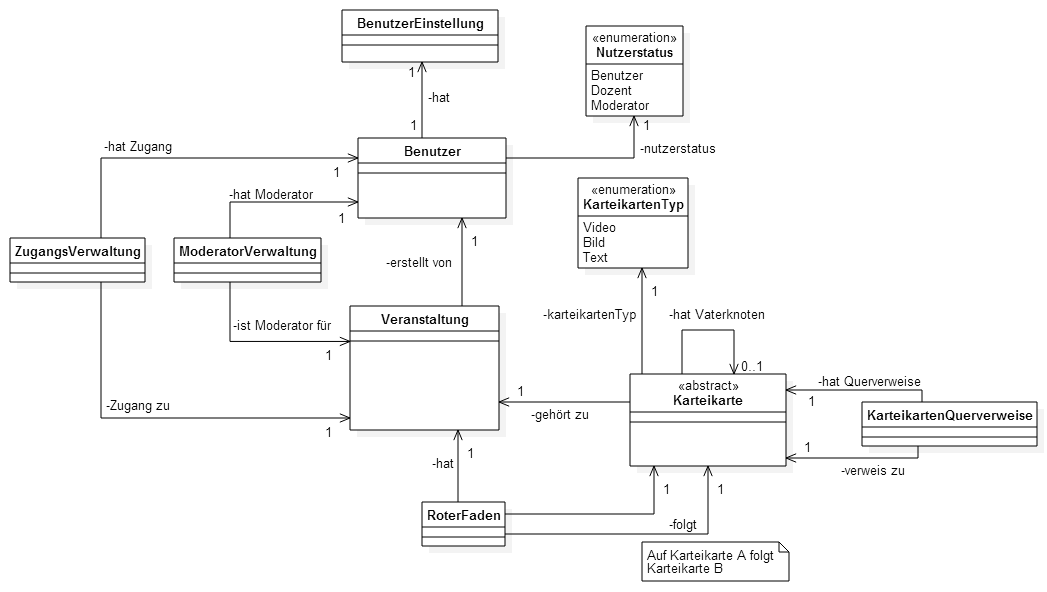
\includegraphics[width=\textwidth]{Bilder/Datenbank/Datenbankentwurf.png}
	\caption{Datenbankdiagramm}
	\label{Datenbankdiagramm}
\end{figure}

\section{Beschreibung der Tabellen}

\begin{tabular}{|lp{12cm}|}
	\hline
	TABELLE			&  Benutzer\\ 
	BESCHREIBUNG	&  Speichert alle Informationen, die zu einem Benutzer gehören.\\ 
	VERWALTET		& Benutzerdaten\\ 
	SCHLÜSSEL		&  ID : Integer\\ 
	\hline
	&  \\ 
	FELD		    &  Vorname : String\\  
	&  \\ 
	FELD		    &  Nachname : String\\  
	&  \\ 
	FELD		    &  Martrikelnummer : Integer\\  
	&  \\
	FELD		    &  eMail : String\\ 
	BESCHREIBUNG	&  Veranstaltungsbeschreibung\\
	&  \\
	FELD		    &  Studiengang : Enum\\ 
	BESCHREIBUNG	&  Fremdschlüssel, Benutzer ist bestimmtem Studiengang zugeordnet. Dozenten sind hier keinem Studiengang zugeordnet. Referenziert auf Tabelle Studiengang\\ 
	&  \\
	FELD		    &  Kennwport : String\\ 
	BESCHREIBUNG	&  Speichert das verschlüsselte Passwort des Nutzers \\
	&  \\
	FELD		    &  Nutzerstatus : Enum\\ 
	BESCHREIBUNG	&  Speichert ob Benutzer ein Student oder Dozent ist.\\
	&  \\
	FELD		    &  GruppeneinladungenErlauben : Bool\\ 
	BESCHREIBUNG	&  Speichert ob Benutzer zu Gruppen eingeladen werden kann.\\
	&  \\
	FELD		    &  NotifyDiskussionen : Enum\\ 
	BESCHREIBUNG	&  Speichert wie ein Benutzer über Diskussionen informiert wird.\\
	\hline
\end{tabular}\\\\
\begin{tabular}{|lp{12cm}|}
	\hline
	TABELLE			&  Studiengang\\ 
	BESCHREIBUNG	&  alle Studiengänge an der Universität Ulm\\ 
	VERWALTET		&  Benutzer und deren eingetragenen Studiengang\\ 
	SCHLÜSSEL		&  ID : Integer\\ 
	\hline
	&  \\
	FELD		    &  Studiengang : String\\ 
	BESCHREIBUNG	&  Text der den Studiengang beschreibt.\\
	\hline
\end{tabular}\\\\


\chapter{System-Architektur}

\section{Kommunikationsdiagramme}

\begin{figure}[H]
	\centering
	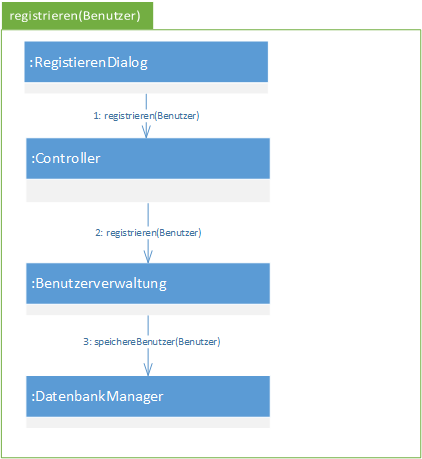
\includegraphics[width=0.7\linewidth]{Bilder/Kommunikationsdiagramme/registrieren}
	\caption{Registrierung}
	\label{Registrierung}
\end{figure}

\begin{figure}[H]
\centering
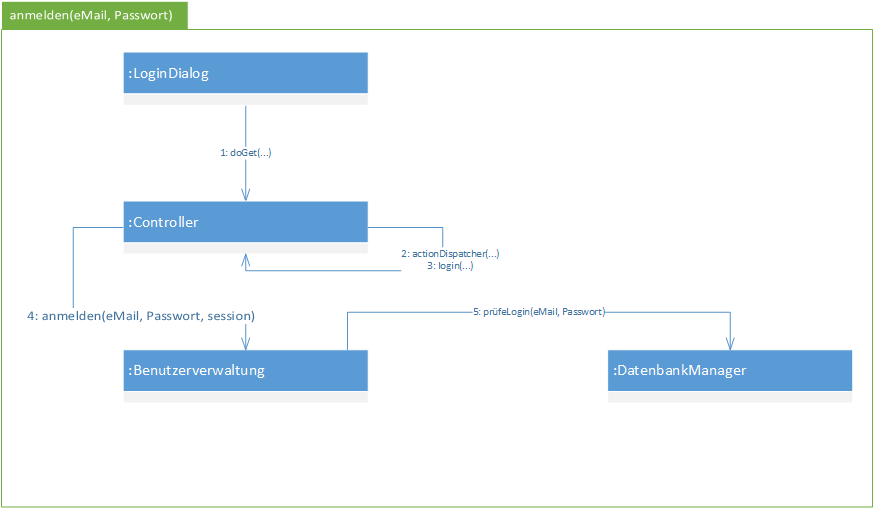
\includegraphics[width=0.7\linewidth]{Bilder/Kommunikationsdiagramme/anmelden}
\caption{Am System anmelden}
\label{Am System anmelden}
\end{figure}


\begin{figure}[H]
\centering
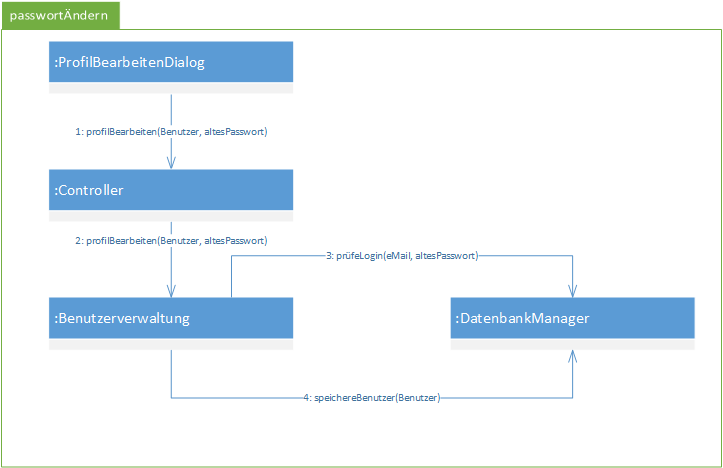
\includegraphics[width=0.7\linewidth]{Bilder/Kommunikationsdiagramme/passwortAendern}
\caption{Passwortänderung}
\label{Passwortaenderung}
\end{figure}


\section{Klassendiagramm}

\begin{figure}[H]
\centering
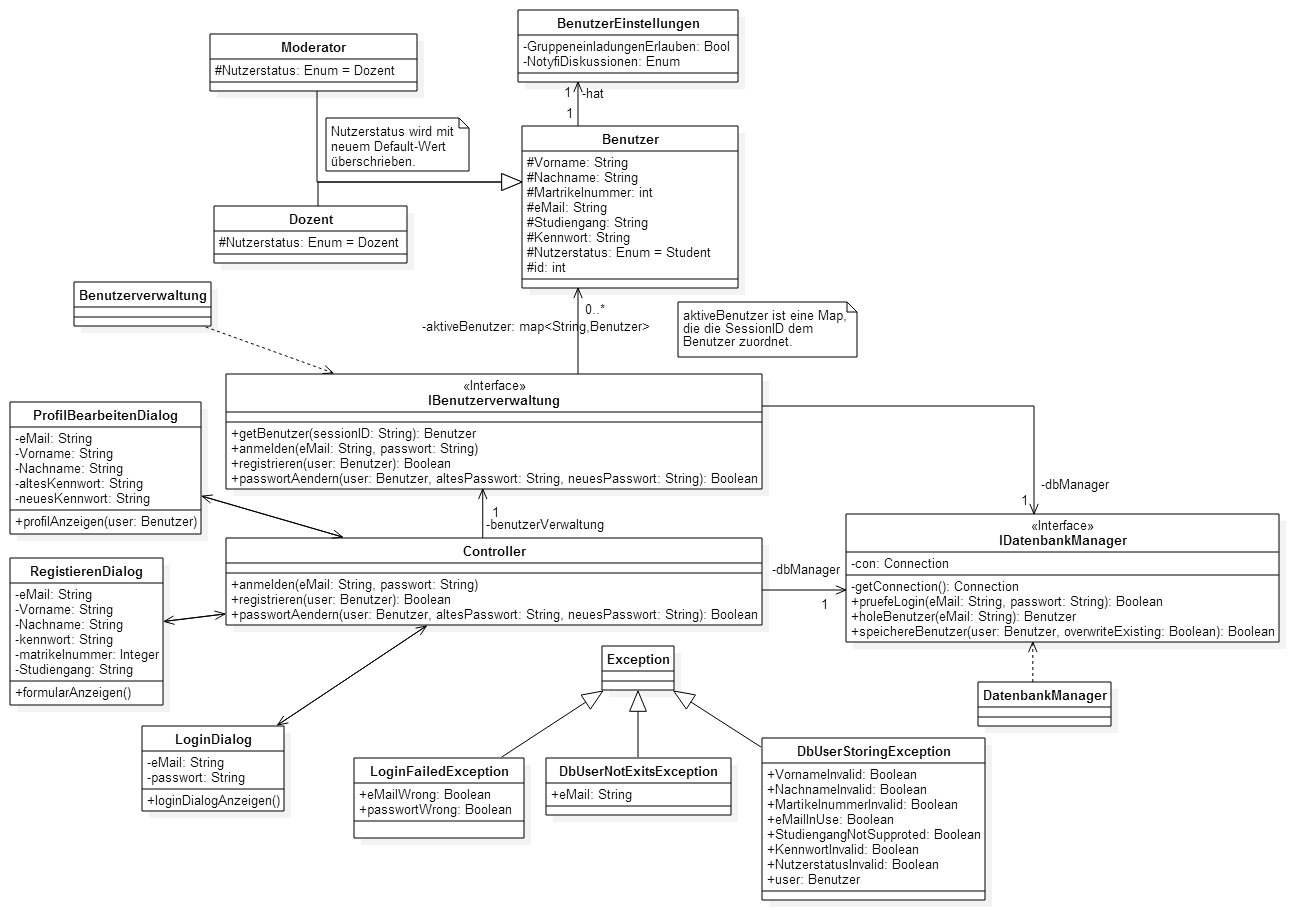
\includegraphics[width=\textwidth]{Bilder/Klassendiagramm/Klassendiagramm}
\caption{}
\label{fig:Klassendiagramm}
\end{figure}


\section{Methodenbeschreibung}
\subsection{Controller Methoden}

\begin{tabular}{|lp{12cm}|}
	\hline
	Operation &  \textbf{anmelden(eMail :String , password: String) }\\ 
	Beschreibung & Methode hier sendet den Aufruf mit den entsprechechenden Daten einfach weiter an die Benutzerverwaltung. \\ 
	\hline 
\end{tabular} \\\\
	

\begin{tabular}{|lp{12cm}|}
	\hline
	Operation &  \textbf{registrieren(user:Benutzer): Boolean) }\\ 
	Beschreibung & Methode hier sendet den Aufruf mit den entsprechechenden Daten einfach weiter an die Benutzerverwaltung. \\ 
	\hline 
	\end{tabular} \\\\

\begin{tabular}{|lp{12cm}|}
	\hline
	Operation &  \textbf{passwortAendern(user:Benutzer, altesPasswort:String, neuesPasswort:String): Boolean) }\\ 
	Beschreibung & Methode hier sendet den Aufruf mit den entsprechechenden Daten einfach weiter an die Benutzerverwaltung. \\ 
	\hline 
\end{tabular} \\\\


\subsection{Benutzerverwaltung  Methoden}

\begin{tabular}{|lp{12cm}|}
	\hline
	Operation &  \textbf{getBenutzer(sessionID:String): Benutzer) }\\ 
	Beschreibung & Liefert das Benutzerobjekt zur entsprechenden Session-ID zurück. Wenn die Benutzerverwaltung diese SessionID nicht kennt ist der Benutzer nicht angemeldet und es wird null zurückgeliefert. Die Benutzerverwaltung merkt sich die Zuweisung zwischen SessionID und eMail-Adresse und kann somit über den DatenbankManager den gewünschten Benutzer übergeben. \\ 
	\hline 
\end{tabular} \\\\


\begin{tabular}{|lp{12cm}|}
	\hline
	Operation &  \textbf{anmelden(eMail:String, passwort:String) }\\ 
	Beschreibung & Auf Grundlage von der SessionID Benutzer-eMail und dem dazugehörigen Passwort wird der Benutzer an dem System angemeldet.\\ 
	\hline 
\end{tabular} \\\\

\begin{tabular}{|lp{12cm}|}
	\hline
	Operation &  \textbf{registrieren(user:Benutzer): Boolean) }\\ 
	Beschreibung & Registrierung bekommt einen Benutzerobjekt mit allen Attributen die im Klassendiagamm dargestellt sind.Falls der Benutzer noch nicht existiert wirde dieser neun in der Datenbank angelegt. \\ 
	\hline 
\end{tabular} \\\\

\begin{tabular}{|lp{12cm}|}
	\hline
	Operation &  \textbf{passwortAendern(user:Benutzer, altesPasswort:String, neuesPasswort:String): Boolean }\\ 
	Beschreibung & \\ 
	\hline 
\end{tabular} \\\\


\subsection{Datenbankmanager  Methoden}
\begin{tabular}{|lp{12cm}|}
	\hline
	Operation &  \textbf{getConnection(): Connection}\\ 
	Beschreibung & \\ 
	\hline 
\end{tabular} \\\\

\begin{tabular}{|lp{12cm}|}
	\hline
	Operation &  \textbf{pruefeLogin(eMail:String, passwort:String): Boolean}\\ 
	Beschreibung & \\ 
	\hline 
\end{tabular} \\\\

\begin{tabular}{|lp{12cm}|}
	\hline
	Operation &  \textbf{holeBenutzer(eMail:String): Benutzer}\\ 
	Beschreibung & \\ 
	\hline 
\end{tabular} \\\\

\begin{tabular}{|lp{12cm}|}
	\hline
	Operation &  \textbf{speichereBenutzer(user:Benutzer, overwriteExisting:Boolean): Boolean}\\ 
	Beschreibung & \\ 
	\hline 
\end{tabular} \\\\


\subsection{RegistrierenDialog  Methoden}

\begin{tabular}{|lp{12cm}|}
	\hline
	Operation &  \textbf{formularAnzeigen()}\\ 
	Beschreibung & \\ 
	\hline 
\end{tabular} \\\\

\paragraph{LoginDialog  Methoden}\mbox{}\\

\begin{tabular}{|lp{12cm}|}
	\hline
	Operation &  \textbf{loginDialogAnzeigen()}\\ 
	Beschreibung & \\ 
	\hline 
\end{tabular} \\\\


\subsection{ProfilBearbeitenDialog  Methoden}

\begin{tabular}{|lp{12cm}|}
	\hline
	Operation &  \textbf{profilAnzeigen(user:Benutzer)}\\ 
	Beschreibung & \\ 
	\hline 
\end{tabular} \\\\

\end{document}
